\documentclass[a4paper,11pt,twoside]{book}
\usepackage[inner=4.2cm,outer=3.0cm,top=1.5in,bottom=1.75in]{geometry}
\usepackage[utf8]{inputenc} %kodowanie znakow
\usepackage[polish]{babel}
\usepackage[T1]{fontenc} %polskie fonty
\usepackage{graphicx}
\usepackage{fancyhdr} % headery i footery
\frenchspacing %likwiduje powiekszone spacje po koncu zdania
\usepackage{ucs} % co to?
\usepackage{amsmath} %do wzorow matematycznych
\usepackage{amsfonts} %---------||--------------
\usepackage{indentfirst} %wciecie pierwszego akapitu
\usepackage{fancyhdr}
\usepackage{clrscode} % jak z Cormena


\newenvironment{packed_enum}{
\begin{enumerate}
  \setlength{\itemsep}{1pt}
  \setlength{\parskip}{0pt}
  \setlength{\parsep}{0pt}
}{\end{enumerate}}



\begin{document}
\pagestyle{fancy}
\fancyhf{}
\lhead{\chaptername{} \thechapter}
\rhead{\thepage}
\cfoot{
\centering
\includegraphics[width=5in]{stopka_loga_napis}
}
\include{tytul}

\chapter{Wstęp}
%\pagestyle{headings} % wlacza numerowanie stron
Witamy Państwa na ćwiczeniach z~Modelowania Molekularnego 2.\\

Zacznijmy od kwestii formalnych. Skrypt zawiera przede wszystkim opis trzech programów zaliczeniowych. Na ćwiczeniach będą one omawiane i~oceniane.
Przystąpienie do egzaminu jest możliwe jedynie po zaliczeniu ćwiczeń. Warunkiem dostatecznym i~koniecznym do uzyskania zaliczenia ćwiczeń jest oddanie samodzielnie napisanych i~działających programów zaliczeniowych, oraz przedstawienie wyników.
W~przypadku oddania wymaganych programów w~wyznaczonych terminach ocena z~przedmiotu zostaje podniesiona o~pół stopnia (gdy oceną z~egzaminu nie jest ani 2.0, ani 5.0). Można więc uznać, że ocena z~ćwiczeń jest ,,zero-jedynkowa''. Zachęcamy Państwa do podjęcia trudu i~uzyskania z~ćwiczeń ,,jedynki''!\\

Uczestników kursu (czyli głównych odbiorców tego skryptu) cechuje duże zróżnicowanie zarówno pod względem umiejętności programistycznych, jak i~pod względem zrozumienia zagadnień fizycznych.
Jednak od wszystkich studentów oczekujemy znajomości podstawowych algorytmów, pojęć programowania obiektowego, jak również znajomości obiektowego języka programowania (Javy, bądź Pythona). Opracowując programy zaliczeniowe braliśmy pod uwagę osoby, które nie miały jeszcze okazji nabyć swobody w~posługiwaniu się podstawowymi narzędziami programistycznymi i~chcemy zapewnić, że choć przewidziany na ćwiczenia materiał nie należy do najprostszych, to trudności techniczne będzie można pokonać systematyczną pracą i~konsultacjami z~ćwiczeniowcem. \\

Skrypt pisany był z myślą o zajęciach prowadzonych przez jeden semestr w wymiarze 60-godzinnym.
Jeżeli założyć, że studenci rozpoczynający ten kurs znają obiektowy język programowania, 60 godzin ćwiczeń wystarczyć powinno do zrealizowania całego skryptu, czyli trzech programów zaliczeniowych.
Jednak możliwe jest również przeprowadzenie ćwiczeń w~wymiarze 30-godzinnym~--~wówczas od studentów wymagać można dwóch pierwszych programów, bądź: pierwszego i trzeciego.\\

Na początku zajmiemy się dynamiką molekularną (\emph{Molecular Dynamics,} MD). {\bf Pierwszy program zaliczeniowy} jest implementacją prostej dynamiki molekularnej. Aby uprościć początkowe rozważania ograniczymy się do układu, składającego się z~pojedynczej cząstki, z~opisem 1-wymiarowym. Cząstka uwięziona będzie w~studni z~dwoma minimami, z~barierą między nimi. Na takim układzie będziemy testować różne algorytmy całkujące (Verlet, Velocity Verlet, Leapfrog i~Beeman). Będzie to układ modelowy, który będziemy w~trakcie ćwiczeń rozwijać, umożliwiając zastosowanie:
\begin{packed_enum}
\item dowolnego pola siłowego;
\item dowolnego algorytu całkującego;
\item dowolnej liczby atomów tworzących układ;
\item opisu 1-, 2-, bądź 3-wymiarowego;
\end{packed_enum}

Następnie zajmiemy się metodą Monte Carlo (MC), a~w szczególności~-~algorytmem Metropolisa. W drugim programie zaliczeniowym modelować będziemy układ \emph{w~kontakcie z~termostatem}\footnote{Mówimy też: \emph{w~kontakcie termicznym z~otoczeniem}, bądź: \emph{w~stałej temperaturze}, bądź: \emph{w~zespole kanonicznym}, bądź: \emph{w~zespole \emph{NVT}}.}. Związane z~tym tematem zagadnienia fizyczne są dość złożone i~do pełnego zrozumienia wymagają znajomości mechaniki statystycznej i~termodynamiki. Mamy jednak nadzieję, że zainteresujemy studentów na tyle, by sami zechcieli pogłębiać swą wiedzę na kursach poświęconych tej tematyce.\\

{\bf Drugi program zaliczeniowy} będzie umożliwiał przeprowadzenie symulacji Monte Carlo z~symulowanym wyżarzaniem (\emph{simulated annealing}) i wymianą replik (\emph{Replica Exchange Monte Carlo, REMC}). Będziemy przeprowadzać symulacje dla bardzo prostego modelu białka~-~\emph{modelu HP}. Powinno się Państwu spodobać to, że polimer zwija się do konfiguracji o~niskiej (jak nie najniższej) energii i możnaby ulec wrażeniu, że temu właśnie służy MC. Jednak odszukanie globalnego minimum energii potencjalnej dla modelu HP jest możliwe zwyczajnie poprzez wygenerowanie wszystkich możliwych konfiguracji (co również uczynimy) i~wybranie tej o~najniższej energii. Przekonają się Państwo, że istotą metody Monte Carlo jest próbkowanie zbioru możliwych konfiguracji według pewnego rozkładu prawdopodobieństwa. W przypadku algorytmu Metropolisa jest to rozkład Boltzmanna (opisany wzorem~(\ref{Boltzmann})).\\ 

Kończąc, chcieliśmy szczególnie mocno podkreślić, że choć główną trudnością z~jaką będą musieli zmierzyć się studenci będzie realizacja projektów programistycznych, to istotą proponowanych ćwiczeń jest przedstawienie subtelności fizycznych, wszytych w~symulacje komputerowe układów molekularnych.
\section{Dynamika molekularna} 
Dynamika molekularna może się Państwu wydawać bliska, choćby ze względu na wcześniejszy kurs, \emph{Modelowanie Molekularne I}, w~ramach którego poznali Państwo narzędzie NAMD do przeprowadzania tego typu symulacji. Cząsteczka białka traktowana jest jak układ klasyczny, dla którego dynamika molekularna generuje ciąg \emph{mikrostanów} wykorzystując algorytmy całkujące równania ruchu. Z tak uzyskanego zbioru mikrostanów wyznacza się rozmaite wielkości fizyczne, np. średnią energię układu.\\

Przez {\bf mikrostan} rozumieć będziemy zbiór parametrów w~pełni opisujących jedną realizację układu. W przypadku białka w~ujęciu klasycznym mikrostan określają pędy i~położenia wszystkich atomów. Przez {\bf konfigurację} rozumieć będziemy jedną realizację, opisaną położeniami atomów, bez pędów. Zbiór wszystkich mikrostanów nazywać będziemy {\bf przestrzenią fazową}. Analogicznie, przez {\bf przestrzeń konfiguracyjną} rozumieć będziemy zbiór możliwych konfiguracji układu.\\

Wróćmy do ciągu mikrostanów jako wyniku dynamiki molekularnej. Ciąg mikrostanów nazywać będziemy {\bf trajektorią}. Jest to w~pewnym sensie film z~życia naszego modelu białka. Jednak trajektoria to coś więcej~-~to próba przestrzeni konfiguracyjnej (czyli zbiór kofiguracji), dzięki której wyznaczamy estymatory {\bf wielkości makroskopowych} takie jak: średnia energia, średnia kwadratu energii i~inne. Często stosowanym założeniem jest to, że tego typu estymatory są zgodne z~wartościami mierzonymi w~doświadczeniu, jednak tylko pod warunkiem, że uzyskana próba mikrostanów jest zgodna z~rozkładem Boltzmanna.\\

Rodzi się pokusa, aby ostateczną weryfikacją tego, czy symulacja przebiegła poprawnie stanowił ogląd filmu uzyskanego z~dynamiki molekularnej. Wówczas, o~ile białko zachowuje się zgodnie z~naszymi intuicjami, symulacja jest ,,dobra'', a~wnioski wyniesione z~symulacji~-~poprawne. Jednak czy nasze intuicje dotyczące białek są słuszne?\\

Przykładowo, często spotykana intuicja mówi, że \emph{białko zwija się do stanu natywnego, któremu odpowiada globalne minimum energii potencjalnej.} Stan natywny to postać białka, w~której występuje ono w~organiźmie i~w~której może spełniać swoją biologiczną funkcję. Jednak skąd pomysł, że jest to jedna, konkretna konfiguracja, ta, dla której uzyskujemy globalne minimum energii potencjalnej? 

Z~drugiej strony, inna intuicja podpowiada nam, że białko wykonuje chaotyczne ruchy, niezbędne do wykonania powierzonych mu zadań. Jednak ruchy te, jakkolwiek ,,małe'', wykluczają możliwość, by białko przebywało w~jednej (ustalonej przez minimum energii potencjalnej) konfiguracji.\\

Intuicje te stoją ze sobą w~sprzeczności.\\

W jaki więc sposób białko realizuje swój stan natywny? Skoro nie utrzymuje jednej konfiguracji, to jakie konfiguracje przyjmuje? Które konfiguracje przyjmuje częściej, a~które rzadziej? Co jest przyczyną takiego stanu rzeczy?\\

Na tych ćwiczeniach przyjmiemy założenie, że stan natywny białka jest dobrze opisany rozkładem Boltzmanna\footnote{Liczymy, że uda się ten (teoretyczny) wynik wyprowadzić, ale istotą drugiego programu zaliczeniowego jest badanie konsekwencji tego założenia.}. Tzn. układ przyjmuje konfiguracje z~pewnym prawdopodobieństwem, określonym przez rozkład Boltzmanna (więcej w~rozdziale~3.).\\

\section{Metoda Monte Carlo}
W zasadzie dobrze przeprowadzona symulacja dostarcza nam ,,dobrej'' próby przestrzeni konfiguracyjnej. Dobrej, ale nie tylko dlatego, że obejrzawszy trajektorię stwierdzamy, że białko wykonuje chaotyczne ruchy, które wydają się ,,sensowne''. Dobre próbkowanie to próbkowanie zgodne z~rozkładem Boltzmanna\footnote{Przynajmniej przy podjętym na tych ćwiczeniach założeniu. Niewykluczone, że przyszłe zastosowania symulacji komputerowych rozszerzą ten ,,paradygmat'', jednak zasady rządzące przeprowadzaniem takich symulacji pozostaną te same, z~dokładnością do rozkładu prawdopodobieństwa, jakim będzie opisany układ.}. Dopiero dla tak wyznaczonej próby możemy wyznaczyć estymatory wielkości makroskopowych białka, które następnie jest sens porównywać z~tymi wyznaczonymi doświadczalnie. Jakie w~takim razie próbkowanie byłoby złe i~prowadziło do błędnie wyznaczonych własności układu? Przykładowo, dla dynamiki liczącej sobie $10^6$ kroków moglibyśmy wyprodukować $10^6$ identycznych kopii pewnej wybranej konfiguracji. Bądź: $10^6$ konfiguracji z~pobliża globalnego minimumum, losowane wg pewnego rozkładu innego niż rozkład Boltzmanna\footnote{Na ćwiczeniach zgłębimy ten przykład i~zobaczymy jak (ewentualnie) wykorzystać dane uzyskane z~drugiego podejścia.}.\\

Zanim przybliżymy Państwu metodę Monte Carlo, chcemy postawić pewien problem. Sama metoda MC z~algorytmem Metropolisa opisana jest w~rozdziale 4., a~najlepiej zaznajomią się z~nią Państwo, implementując drugi program zaliczeniowy.\\

W poprzednim paragrafie wspomnieliśmy o~stanie natywnym białka. Warto wiedzieć, że istnieją tzw. \emph{natywnie nieustrukturalizowane białka} (\emph{natively unfolded proteins}). Biolog strukturalny może określić białka z~tej klasy jako ,,nie mające ustalonej struktury''. Białka te natywnie przyjmują bardzo wiele znacznie różniących się między sobą konfiguracji. Nawet gdyby jakieś białko tego typu udało się skrystalizować i~określić strukturę jednego z~mikrostanów, to ciężko oczekiwać, by o~własnościach tego białka można było wnioskować na podstawie tej jednej konfiguracji. Szacuje się, że blisko 30\% eukariotycznych białek zalicza się do tej klasy, bądź zawiera regiony o~nieokreślonej strukturze~\cite{unfolded}.\\

Co mogłoby być przyczyną tego, że białko ,,nie chce przebywać'' w~pobliżu globalnego minimum energii potencjalnej? Innymi słowy: co sprawia, że białko zasługuje na miano natywnie nieustukturalizowanego? Czy to, że takie minimum nie istnieje? Być może białko nie jest w~stanie go osiągnąć? Czy może posiada wiele konfiguracji o~niskiej energii, ale żadna z~nich nie ,,przeważa'' w~istotny sposób? Odpowiedzi na te pytania uzyskają Państwo implementując metodę Monte Carlo z~algorytmem Metropolisa w~ramach drugiego programu zaliczeniowego.
\chapter{Pierwszy program zaliczeniowy}
Wraz ze skryptem otrzymali Państwo szkic programu do przeprowadzania dynamiki molekularnej. Pierwsze laboratoria poświęcimy omówieniu klas zdefiniowanych w~tym programie. Jednak zachęcamy Państwa do samodzielnego zaprojektowania i~implementacji programu.  
\section{Zarys programu}
Będziemy zajmować się klasycznym opisem układu, w~którym ewolucję $i$-tego atomu opisuje II zasada dynamiki Newtona:
\begin{equation}
\ddot{\mathbf{r}}_i = \frac{1}{m_i} \mathbf{F}_i,\label{IIzasada}
\end{equation}
gdzie $m_i$ jest masą, $\ddot{\mathbf{r}}_i$ przyspieszeniem, zaś $\mathbf{F}_i$~-~siłą działającą na ten atom.\\

Znane Państwu dobrze z~liceum równanie (\ref{IIzasada})~jest opisem układu izolowanego, w~którym położenia atomów wyrażone są we współrzędnych kartezjańskich. W~bardziej zaawansowanych (i~w~praktyce: częściej stosowanych) podejściach układ opisany jest współrzędnymi uogólnionymi, a~ewolucję układu wyrażają równanie Eulera-Lagrange'a, bądź równania Hamiltona. Jednak dużo ważniejszą uwagą jest ta, że równanie (\ref{IIzasada})~opisuje układ izolowany\footnote{Nie wymieniający z~otoczeniem ani energii, ani materii. W~takim układzie zachowana jest energia, tzn. $E_{całkowita}(t)=const$.}, natomiast białko takim układem $NIE$ jest.\\

W~pierwszym programie zaliczeniowym ograniczymy się do układów izolowanych. Na ćwiczeniach postaramy się przybliżyć Państwu tematykę związaną z~modelowaniem układów w~kontakcie termicznym z~otoczeniem.\\

W celu uzyskania trajektorii wszystkich atomów, $\mathbf{r}(t)$, należałoby rozwiązać układ równań różniczkowych II stopnia~-~równań (\ref{IIzasada})~-~co w~przypadku podejścia analitycznego jest zazwyczaj bardzo złożonym problemem. Natomiast numeryczna procedura jest stosunkowo prosta i~przedstawia się następująco (zapożyczone z~\cite{understanding}):
\begin{codebox}
\Procname{$\proc{Prosta-Dynamika-Molekularna}$}
	\li $\id{U}\gets\proc{Inicjalizacja}$ 
	\li \Comment Zainicjalizuj układ $U$
	\li $\id{t} \gets 0$
	\li \While $t < \id{tmax}$
	\li \Do
		\li $\proc{Procedura-Wyznaczająca-Siły(\id{U})}$
		\li $\proc{Procedura-Całkująca(\id{U})}$
		\li $\proc{Zapamiętaj-Statystyki(\id{U})}$
		\li $\id{t}\gets t+1$
	\End
	\li $\proc{Wypisz-Statystyki-Do-Pliku}$
\End
\end{codebox}
Analog powyższego znajdą Państwo w~dołączonych do skryptu plikach ze szkicem programu.
\section{Treść pierwszego programu zaliczeniowego}
Zaimplementuj procedurę przeprowadzającą prostą dynamikę molekularną, która wykorzystywać będzie dowolny potencjał i~dowolny algorytm całkujący (w~szczególności~-~potencjały i~algorytmy całkujące omówione dalej).

Symulację ograniczymy do przypadku 1-wymiarowego, ale z~dowolną liczbą atomów. Położenie, prędkość i~przyspieszenie atomu określać będą obiekty klasy \texttt{Vec} z~metodami analogicznymi do operacji wykonywanych na wektorach.

Program powinien pobierać informacje dotyczące:
\begin{packed_enum}
\item używanego potencjału,
\item algorytmu całkującego, 
\item liczby atomów,
\item liczby kroków symulacji,
\item długości kroku czasowego,
\end{packed_enum}
z~linii komend (argument \texttt{args} metody \texttt{main}), bądź z~pliku.

Początkowo wszystkie atomy będą miały zerową prędkość. Położenia początkowe program może wybierać drogą losową, bądź według prostego algorytmu Państwa autorstwa (np. poukładane na osi $x$, w~odleglosci 1 między kolejnymi atomami). Dla uproszczenia rozważmy przypadek, w~którym wszystkie atomy mają tę samą masę równą 1.

Jako wynik program powinien zwracać trajektorię układu (generować plik \texttt{xyz}), oraz zależność energii: potencjalnej, kinetycznej i~całkowitej, od czasu (plik \texttt{csv}). Symulacja powinna być ,,poprawna'' w~tym sensie, że energia układu powinna utrzymywać się na (względnie) stałym poziomie. \\

Na omówienie potencjałów i~algorytmów całkujących poświęcamy resztę tego rozdziału, jak również ćwiczenia i~laboratoria.
\section{Energia potencjalna}
Zakładamy, że energia potencjalna jest funkcją (jedynie) położeń atomów (czyli konfiguracji układu), $U=U(\mathbf{r})$, a~siła działająca na $i$-ty atom wyraża się następująco:
\begin{displaymath}
\mathbf{F}_i = -\frac{\partial U}{\partial \mathbf{r}_i}
\end{displaymath}
Zatem przyjmujemy założenie, że funkcja energii potencjalnej jest różniczkowalna.
\subsection{Miękkie ścianki}
Najprostszy potencjał gwarantujący, że układ nam ,,nie ucieknie'' to potencjał imitujący ,,miękkie ścianki''. Energia potencjalna $i$-tego atomu zależy od jego odległości od początku układu współrzędnych:
\begin{displaymath}
U(\mathbf{r}_i) = \left\{ \begin{array}{ll}
0 & \textrm{, jeżeli $r_i<L$}\\
\frac{1}{2}f(L-||\mathbf{r}_i||)^2 & \textrm{, wpp}
\end{array} \right.
\end{displaymath}
gdzie $f$~to~stała determinująca ,,twardość'' ścianek, zaś $L$~-~rozmiar wnęki o~energii potencjalnej zero.
\subsection{Potencjał ,,minimum-bariera-minimum''}
Będziemy przeprowadzać symulacje dla 1-wymiarowego atomu uwięzionego w~studni o~dwóch minimach. Wykorzystamy poniższy potencjał:
\begin{displaymath}
U(x)=-a e^{-b (x-1)^2}-c e^{-(x+1)^2}+d x^4,
\end{displaymath}
z~parametrami $a=5$, $b=10$, $c=3$, $d=0,02$. Przy takim zestawie parametrów wykres energii potencjalnej przedstawia Rys. 2.1.
\begin{figure}[h!]
\label{potencjal}
\caption[To należy zmienić]
{
Potencjał ,,minumum-bariera-minimum'':\\
\centering
$U(x)=-5 e^{-10 (x-1)^2}-3 e^{-(x+1)^2}+0,02 x^4$
}
\centering
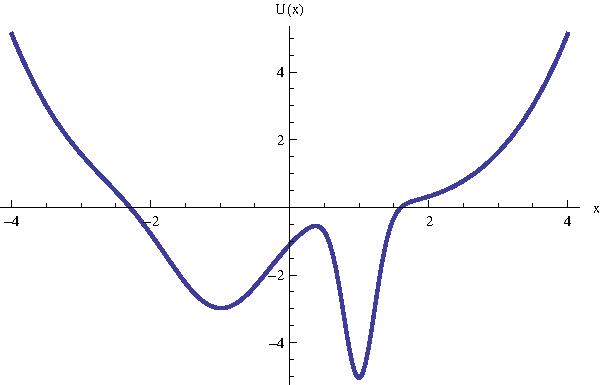
\includegraphics[scale=0.9]{weberPotential}
\end{figure}
To na co warto zwrócić uwagę, to że ,,lej'' po lewej jest płytszy, ale szerszy od tego po prawej. Na ćwiczeniach zbadamy gęstość rozkładu Boltzmanna takiego potencjalu, $\rho (x)\sim e^{-U(x)/k_BT}$, i~wyciągniemy wnioski odnośnie tego, w~którym ,,leju'' atom będzie częściej przebywał.
\subsection{Potencjał Lenarda-Jonesa}
Na ćwiczeniach stosować będziemy tylko jeden potencjał przedstawiający oddziaływanie pary atomów~-~potencjał Lenarda-Jonesa:
\begin{displaymath}
U(\mathbf{r}_{ij}) = \mathcal{E} \left [ \left ( \frac{R}{\mathbf{r}_{ij}} \right )^{12} - 2 \left ( \frac{R}{\mathbf{r}_{ij}} \right )^6  \right ],
\end{displaymath}
gdzie $\mathbf{r}_{ij}$ to odległość między atomami $i$~oraz $j$, zaś $R$ i~$\mathcal{E}$ to parametry potencjału. Wystarczające będzie dla nas ustalenie stałych wartości parametrów, przykładowo $R=1$, $\mathcal{E}=1$.
\section{Algorytmy całkujące}
Algorytm całkujący pozwala wyznaczyć następne (w~chwili czasu $t+\Delta t$) położenia i~prędkości atomów, na podstawie poprzednich położeń, prędkości i~przyspieszeń (w~chwilach czasu $t$, $t-\Delta t$, $t-2\Delta t$, bądź dalszych, w~zależności od złożoności algorytmu).\\

Algorytmy nie będą omawiane w~tym skrypcie, a~jedynie prezentowane w~sposób umożliwiający szybką implementację.
\subsection{Algortm Verleta}
To nasz algorytm wyjściowy. Najprostszy w~implementacji i~stabilny.
\begin{displaymath}
\mathbf{r}(t+\Delta t) := 2\mathbf{r}(t) - \mathbf{r}(t-\Delta t) + \mathbf{a}(t)\Delta t^2,
\end{displaymath}
przy czym znak ,,$:=$'' należy interpretować jako ,,przypisz wartość'' czy też ,,staje się'', znane Państwu z~praktyki programistycznej. Jest to konwencja obowiązująca do końca tego rozdziału.\\

Prędkość nie jest potrzebna do wyznaczenia nowych położeń, ale niezbędna do obliczenia energii kinetycznej. Można ją obliczyć (estymować) następująco:
\begin{displaymath}
\mathbf{v}(t) := \frac{\mathbf{r}(t)-\mathbf{r}(t-\Delta t)}{\Delta t},
\end{displaymath}
\subsection{Velocity Verlet}
Składa się z~dwóch kroków:
\begin{displaymath}
\mathbf{v}(t+\Delta t) := \mathbf{v}(t) + \frac{\mathbf{a}(t-\Delta t)+\mathbf{a}(t)}{2} \Delta t
\end{displaymath}
oraz:
\begin{displaymath}
\mathbf{r}(t+\Delta t) := \mathbf{r}(t) + \mathbf{v}(t+\Delta t)\Delta t + \frac{\mathbf{a}(t)}{2}\Delta t^2
\end{displaymath}
\subsection{Leapfrog}
Na algorytm \emph{leapfrog} również składają się dwa kroki:
\begin{displaymath}
\mathbf{v}(t+\Delta t) := \mathbf{v}(t) + \mathbf{a}(t)\Delta t
\end{displaymath}
oraz:
\begin{displaymath}
\mathbf{r}(t+\Delta t) := \mathbf{r}(t) + \mathbf{v}(t+\Delta t)\Delta t
\end{displaymath}
\chapter{Układ w~kontakcie z~termostatem}
\section{Rozkład Boltzmanna}
Rozkład Boltzmanna, opisujący układ o~stałej temperaturze $T$, wyraża prawdopodobieństwo tego, że układ znajdzie się w~$i$-tej konfiguracji\footnote{Ta postać rozkładu Boltzmanna sformułowana jest dla układu o~przeliczalnym zbiorze możliwych konfiguracji.}:
\begin{equation}
p(i) = \frac{1}{Z} \exp [−E(i)/k_B T ], \label{Boltzmann}
\end{equation}
gdzie $E(i)$ to energia $i$-tej konfiguracji, $k_B$ to stała Boltzmanna, a~stała normalizacyjna $Z$ zapewnia normalizację rozkładu:
\begin{displaymath}
\sum_{i=1}^N p(i) = \frac{1}{Z} \sum_{i=1}^N \exp [ -E(i)/k_B T ]= 1
\end{displaymath}
skąd:
\begin{displaymath}
Z = \sum_{i=1}^N \exp [-E(i) / k_B T],
\end{displaymath}
gdzie $N$ jest liczbą konfiguracji jakie może przyjąć układ. Niestety, stała $Z$ jest praktycznie niemożliwa do wyznaczenia dla większych układów, co oznacza, że nie jesteśmy w~stanie podać explicite prawdopodobieństw poszczególnych konfiguracji.\\

Na początku wspomnieliśmy, że gdybyśmy umieli odtworzyć przestrzeń konfiguracyjną układu, moglibyśmy wyznaczyć jego własności fizyczne. Dużo bardziej zaskakujące jest to, że wszystkie własności makroskopowe układu (a one nas zwykle interesują) bylibyśmy w~stanie wyznaczyć, gdybyśmy umieli wyznaczyć stałą normalizacyjną $Z$, występującą w~rozkładzie Boltzmanna\footnote{W rzeczywistości $Z$ jest funkcją parametrów układu i~nazywa się ją często \emph{sumą statystyczną}.}!
\section{Własność makroskopowa}
Najpierw podamy podejście bardziej ogólne,
w którym przestrzeń fazowa jest zbiorem gęstym, a~nie przeliczalnym. Poniższy akapit nie jest związany z~modelem HP, ale polecamy go Państwa uwadze.\\

Mikrostan układu oznaczymy przez $\mathbf{x} = (\mathbf{p}, \mathbf{q})$, gdzie $\mathbf{p}$ to pędy uogólnione, a~$\mathbf{q}$~to współrzędne uogólnione~-~razem opisują one jedną realizację układu. Niech $A$~będzie pewną własnością fizyczną badanego układu, przykładowo: energią potencjalną. Dla mikrostanu $\mathbf{x}_i$ własność $A$~przyjmuje wartość $A(\mathbf{x}_i)$. Przyjmujemy, że wartość $A$~mierzona w~doświadczeniu (tzw. {\bf własność makroskopowa}) jest równa wartości oczekiwanej $\mathbb{E} A$ przy zadanej gęstości prawdopodobieństwa $f$, tzn.:
\begin{displaymath}
\mathbb{E} A = \lambda Z^{-1} \int_{\Omega} A(\mathbf{x}) f(\mathcal{H}(\mathbf{x}),T) d\mathbf{x}
\end{displaymath}
gdzie $\lambda$ jest stałą, $T$ to temperatura, $\mathcal{H}$ to hamiltonian układu, a~$\Omega$ jest przestrzenią fazową, zaś:
\begin{displaymath}
Z = \int_{\Omega} f(\mathcal{H}(\mathbf{x}),T) d\mathbf{x}
\end{displaymath}
to suma statystyczna (nazwana również \emph{funkcją podziału}). Istotne jest, aby zechcieli Państwo zauważyć, że $f$ jest funkcją (jedynie!) energii całkowitej układu i~temperatury\footnote{Tak jest w~przypadku, gdy jedyne oddziaływanie układu z~otoczeniem to oddziaływanie termiczne.}.\\

W przypadku modelu HP (którego dotyczy drugi program zaliczeniowy) liczba mikrostanów układu jest skończona (ozn. $N$), zaś wartość oczekiwana $A$~wyraża się w~postaci sumy po dostępnych mikrostanach układu:
\begin{equation}
\mathbb{E} A = \sum_{i=1}^N A(i) p(i),\label{oczekiwana}
\end{equation}
gdzie $p(i)$ jest prawdopodobieństwem $i$-tego mikrostanu. Prawdopodobieństwo, że układ o~określonej, stałej temperaturze $T$~znajdziemy w~$i$-tym mikrostanie o~energii $E_i$, dane jest rozkładem Boltzmanna, który dla utrwalenia zapiszemy jeszcze raz, w~nieco innej postaci:
\begin{equation}
p(i) = \frac{\exp [ -E(i)/k_B T ]}{\sum_{j=1}^N \exp [ -E(j)/k_B T ]} .
\end{equation}
Suma w~mianowniku zapewnia normalizację rozkładu $p$:
\begin{displaymath}
\sum_{k=1}^N p(k) =1.
\end{displaymath}
\section{Metoda Monte Carlo (słowem wstępu)}
Metoda Monte Carlo z~algorytmem Metropolisa pozwala nam próbkować konfiguracje układu zgodnie z~rozkładem Boltzmanna, nawet jeżeli nie jesteśmy w~stanie wyznaczyć stałej $Z$.\\

Powiedzieliśmy we wstępie, że implementując drugi program zaliczeniowy uzyskają Państwo odpowiedź na pytanie: \emph{dlaczego} białka natywnie nieustrukturalizowane nie przyjmują jednej konfiguracji. Odpowiedź zawarta jest we wzorze (\ref{Boltzmann}), a~to, że dojście do niej wymaga obycia się z~rozkładem Boltzmanna pokazuje jak piękne potrafią być proste odpowiedzi na złożone pytania.\\
\chapter{Drugi program zaliczeniowy}
\section{Model HP}
Model HP (\emph{hydrophobic-polar protein folding model}) to model polimeru wykorzystywany w~badaniach nad ogólnymi zasadami rządzącymi procesem zwijania białek. Badania tego typu w~przypadku modeli pełnoatomowych wiążą się ze znacznymi kosztami obliczeniowymi, podczas gdy w~modelu HP, ze względu na uproszczoną charakterystykę układu, możliwe jest przeprowadzenie krótkiej symulacji (trwającej od kilku minut do kilku godzin), w~trakcie której układ jest w~stanie osiągnąć wszystkie możliwe konfiguracje.
\begin{figure}[h!]
\label{transformacja}
\centering
\caption[cokolwiek]{
Dwuwymiarowy model HP o~sekwencji: HPHPHHHHHPHP (wizualizacja w~PyMOLu). Na czerwono zaznaczono aminokwasy hydrofobowe (H), na czarno aminokwasy polarne (P).\\
{\bf Po lewej:} Ponieważ nie występują kontakty H-H, energia wynosi 0.\\
{\bf Środkowy:} Obrót wokół szóstego aminokwasu (zaznaczono na zielono) skutkuje utworzeniem kontaktu H-H między ósmym i~piątym aminokwasem. \\
{\bf Po prawej:} Transformacja została zaakceptowana, liczba kontaktów H-H wynosi 1, zatem nowa energia układu wynosi $-\epsilon$.
}
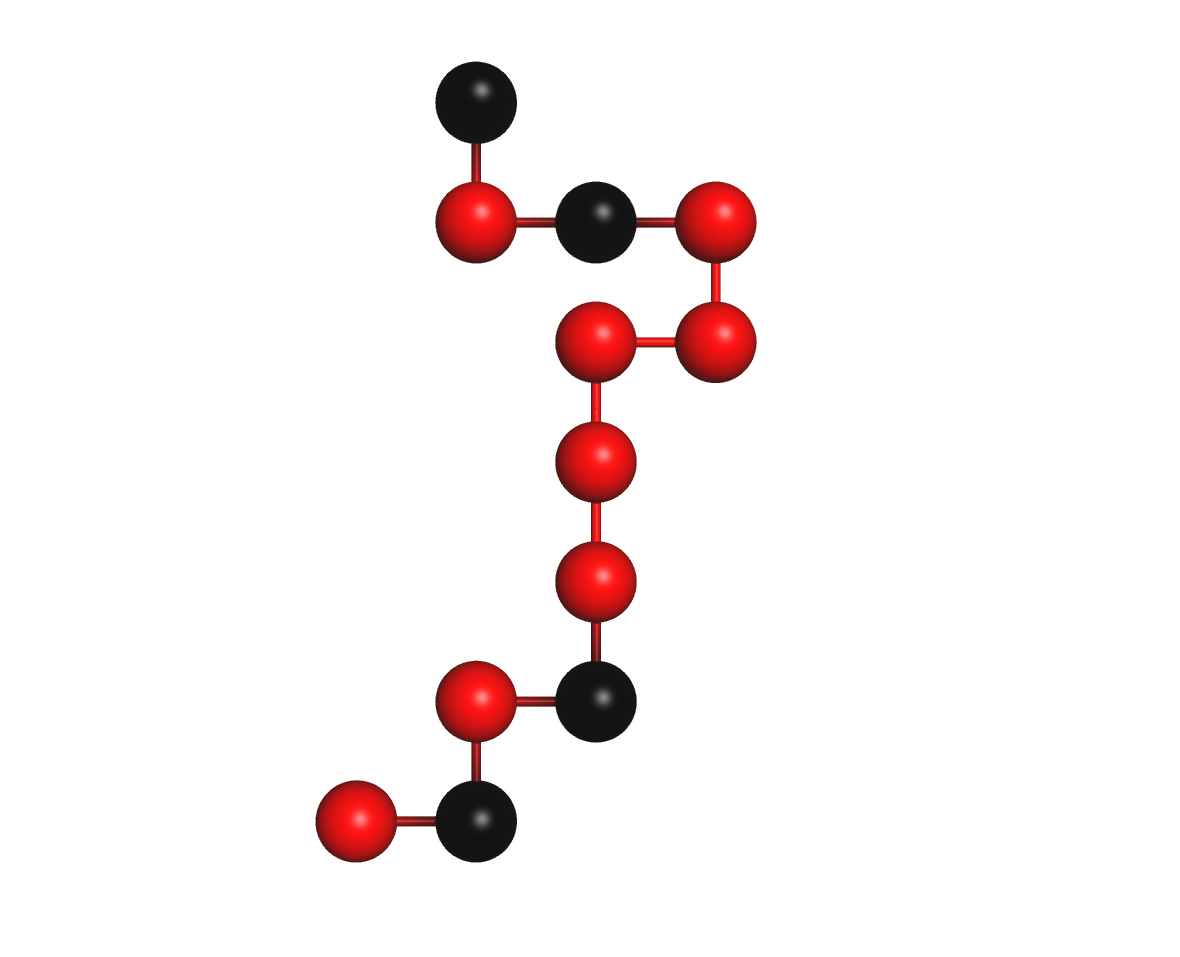
\includegraphics[width=.3\textwidth]{Hp2d2_1}
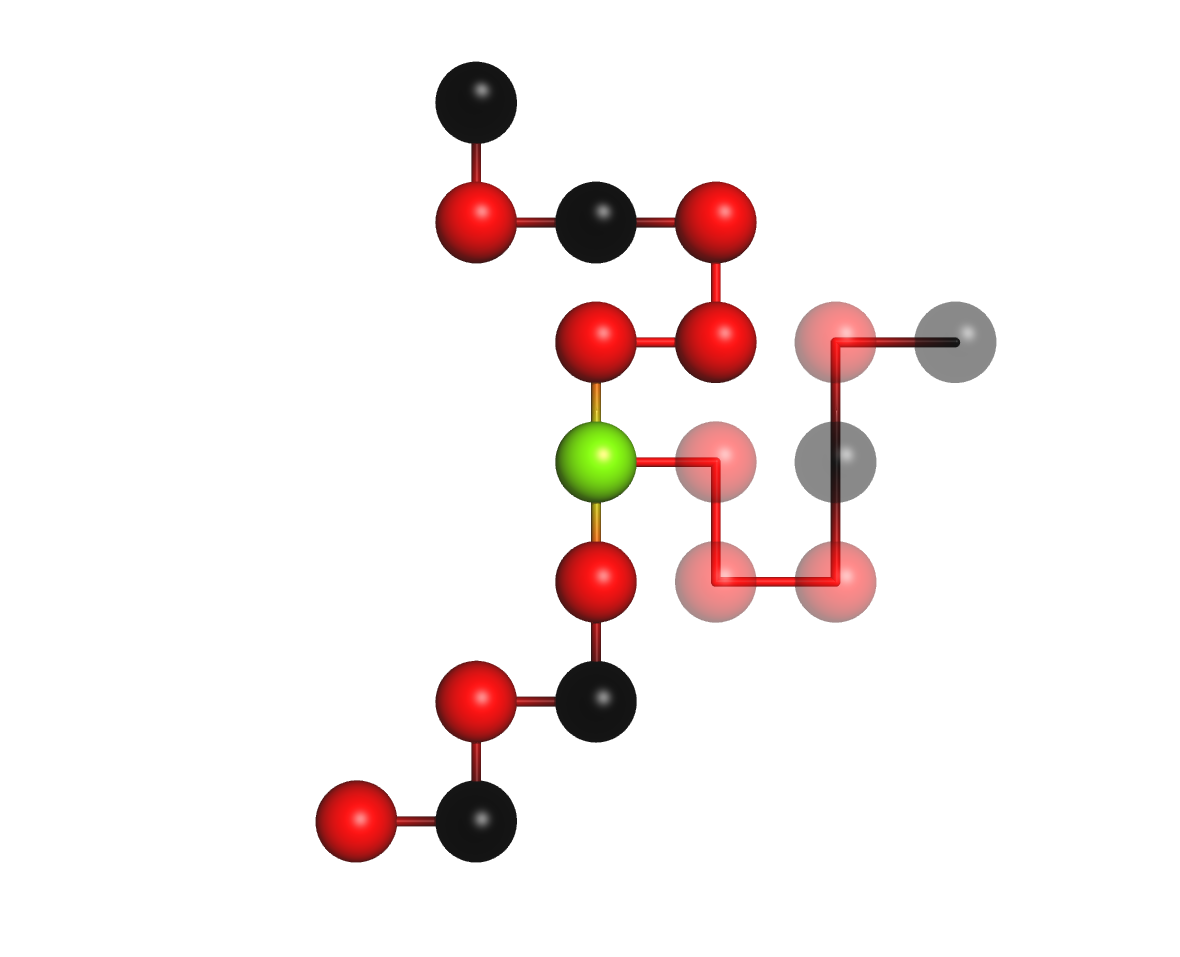
\includegraphics[width=.3\textwidth]{Hp2d2_inter}
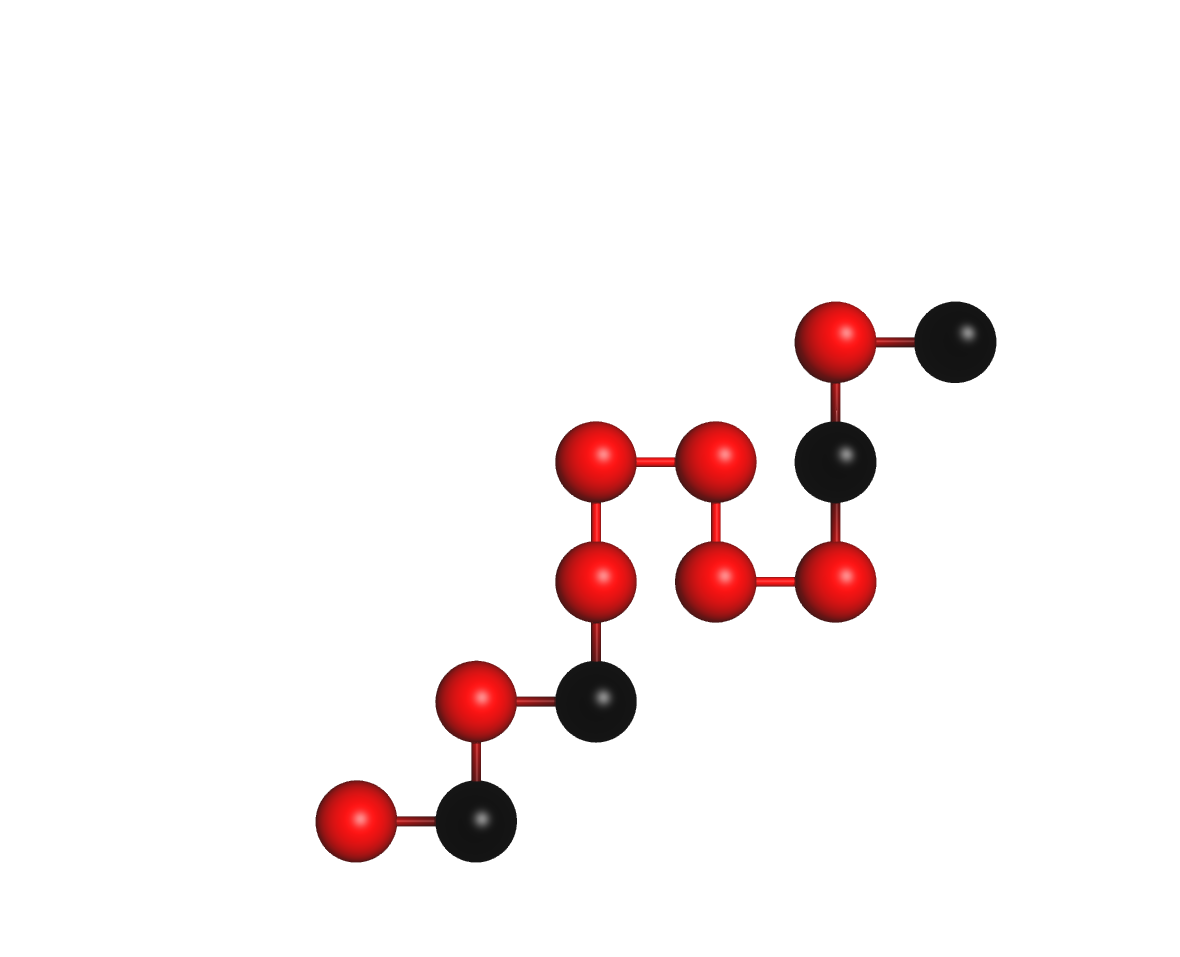
\includegraphics[width=.3\textwidth]{Hp2d2_2}
\end{figure}

Idea modelu HP opiera się na obserwacji, iż kluczową rolę w~procesie zwijania białek pełni efekt hydrofobowy (w~tym kontekście spotkać się można z~terminem: ,,oddziaływania hydrofobowe''). W podstawowym modelu HP polimer zbudowny jest z~monomerów H (hydrofobowych) oraz P (polarnych), przy czym wkład do energii pochodzi jedynie od H. Można więc myśleć o~modelu HP jak o~modelu białka, w~którym alfabet aminokwasów ograniczony został do zbioru $\{H, P \}$. Aminokwasy znajdują się w~węzłach sieci kwadratowej (\emph{square lattice}) w~przypadku modelu dwuwymiarowego, zaś w~przypadku modelu trójwymiarowego~-~w~węzłach sieci sześciennej (\emph{cubic lattice}). Dwa aminokwasy nie mogą znajdować się w~tym samym węźle. Natomiast jeśli dwa aminokwasy połączone są wiązaniem (przez analogię do wiązania peptydowego między aminokwasami w~białkach), to muszą się one znajdować w~sąsiednich węzłach. Mikrostan układu można określić poprzez: sekwencję peptydu oraz położenia poszczególnych aminokwasów (czyli konfigurację).\\

Ewolucję układu w~modelu HP zadają:
\begin{packed_enum}
\item zestaw transformacji struktury;
\item prawdopodobieństwa przejść między mikrostanami.
\end{packed_enum}
Przykładem transformacji może być obrót części białka o~pewien kąt wokół wybranego aminokwasu (Rys.~\ref{transformacja}). W przypadku modelu 2D istnieją cztery możliwe obroty, z~czego jeden z~nich jest przekształceniem identycznościowym. Jeżeli po dokonaniu obrotu żadne dwa aminokwasy nie zajmują tego samego punktu w~przestrzeni, obrót uznajemy za \emph{dozwolony}.\\

Po dokonaniu dozwolonej transformacji, prawdopodobieństwo akceptacji nowego mikrostanu zależy jedynie od zmiany wartości energii, $\Delta E = E_{nowa} −E_{stara}$. Innymi słowy: to czy zaakceptujemy transformację zależy jedynie od tego jaki jest ,,nowy'' i ,,stary'' mikrostan~-~wcześniejsza historia układu nie ma tu znaczenia. Zatem ewolucja peptydu (ciąg konfiguracji wygenerowany w~toku symulacji) jest realizacją procesu stochastycznego, w~którym prawdopodobieństwo akceptacji nowej konfiguracji zależy jedynie od tego, jaka była poprzednia\footnote{Proces stochastyczny w~którym prawdopodobieństwa zdarzeń zależą jedynie od ,,stanu przed'' i~,,stanu po'' nazywany jest \emph{łańcuchem Markowa}.}.\\
\section{Sieć}
Niech:
\begin{displaymath}
\mathbf{e}_x = (1,0), \quad \mathbf{e}_y = (0,1)
\end{displaymath}
będą wektorami bazowymi w~przypadku dwuwymiarowym, zaś:
\begin{displaymath}
\mathbf{e}_x = (1,0,0),\quad \mathbf{e}_y = (0,1,0),\quad \mathbf{e}_z = (0,0,1)
\end{displaymath}
wektorami bazowymi w~przypadku trójwymiarowym. Siecią kwadratową nazywać będziemy zbiór
\begin{displaymath}
LATTICE_{2D} = \{ x\mathbf{e}_x + y\mathbf{e}_y : x, y \in \mathbb{Z}   \}
\end{displaymath}
zaś zbiór:
\begin{displaymath}
LATTICE_{3D} = \{ x\mathbf{e}_x + y\mathbf{e}_y + z~\mathbf{e}_z : x, y,z \in \mathbb{Z}   \}
\end{displaymath}
nazwiemy siecią sześcienną. Element sieci (węzeł) opisujemy przez podanie dwóch, bądź trzech liczb całkowitych (współrzędnych węzła), przykładowo dla sieci sześciennej: (0,1,-10). Powiemy, że węzły $\mathbf{a}$ i~$\mathbf{b}$ sąsiadują ze sobą (ozn. $\mathbf{a} \sim \mathbf{b}$), jeżeli istnieje wektor bazowy $\mathbf{e}$ taki, że:
\begin{displaymath}
\mathbf{a} = \mathbf{b} + \mathbf{e}  \quad \vee \quad \mathbf{b} = \mathbf{a} + \mathbf{e}
\end{displaymath}
Niech $CHAIN = \{1, ..., m\}$ będzie zbiorem aminokwasów tworzących peptyd, gdzie $m$~to długość peptydu. Wówczas strukturę przestrzenną (dla sieci kwadratowej) wyrażać będziemy przez funkcję:
\begin{displaymath}
\mathbf{s} \colon CHAIN \to LATTICE_{2D}
\end{displaymath}
spełniającą warunki 
\begin{displaymath}
\mathbf{s}(1) = (0,0)
\end{displaymath}
\begin{displaymath}
\forall_{i \neq j} \quad \mathbf{s}(i) \neq \mathbf{s}(j)
\end{displaymath}
\begin{displaymath}
\forall_{i<n} \quad \mathbf{s}(i+1) \sim \mathbf{s}(i)
\end{displaymath}

Sama struktura (w postaci funkcji $\mathbf{s}$) nie wystarcza do określenia energii układu, potrzebna jest jeszcze sekwencja aminokwasowa.
\section{Sekwencja}
Sekwencja łańcucha określona jest przez wzorzec hydrofobowy:
\begin{displaymath}
Pat \colon CHAIN \to \{ H, P \}.
\end{displaymath}
Rozważany model dzieli aminokwasy ze względu na właściwości oddziaływań dalekozasięgowych na dwie kategorie: hydrofobowe (H) oraz polarne (P). Dalekozasięgowość oddziaływań odnosi się do wzajemnych położeń aminokwasów w~sekwencji, a~nie w~przestrzeni. Przykładowo: o~obecności oddziaływań dalekozasięgowych możemy mówić w~przypadku pary aminokwasów o~numerach 1 i~4, bądź: 2 i~9, ale nie w~przypadku par: 1 i~3, czy też 4 i~5 (które są ,,blisko siebie'' w~sekwencji). Szczegóły w~poniższej sekcji \emph{Oddziaływania.}
\section{Oddziaływania}
W najprostszym modelu HP rozważa się jedynie oddziaływania dalekozasięgowe pomiędzy aminokwasami hydrofobowymi. Parę aminokwasów hydrofobowych, znajdujących się w~sąsiednich węzłach, które nie są ,,blisko siebie w~sekwencji'', nazwiemy \emph{kontaktem}. Energia danej struktury zależy jedynie od liczby kontaktów i~jest do niej proporcjonalna.\\

Ściślej, niech:
\begin{displaymath}
K_{HH}(\mathbf{s}) = \# \{ \{ i,j \} : \quad |i-j|>2, \quad \mathbf{s}(i) \sim \mathbf{s}(j), \quad Pat(i)=Pat(j)=H\}
\end{displaymath}
oznacza liczbę kontaktów w~strukturze $\mathbf{s}$. Energia układu wyraża się wzorem:
\begin{displaymath}
E(\mathbf{s}) = -\epsilon K_{HH}(\mathbf{s}),
\end{displaymath}
gdzie $\epsilon>0$.\\

Interakcje pomiędzy aminokwasami hydrofobowymi odzwierciedlają ich tendencję do kierowania się do wewnątrz białka i~tym samym unikania kontaktu z~wodą. Należy podkreślić, że model HP uwydatnia jeden aspekt procesu zwijania białek (efekt hydrofobowy), ignoruje natomiast oddziaływania lokalne występujące w~rzeczywistym białku:
\begin{packed_enum}
\item sztywność łańcucha (objawiającą się niedozwolonymi wartościami kątów $\phi$-$\psi$ na wykresie Ramachandrana)
\item wiązania wodorowe (istotne między innymi w~$\alpha$-helisach i~$\beta$-kartkach, czyli w~tzw. strukturze II-rzędowej).
\end{packed_enum}

Model HP jest niezwykle prosty, co nasuwa jedno oczywiste pytanie: \emph{Czy nie jest przypadkiem ZBYT prosty?} Naturalnie, rzeczywiste białka (a~nawet bardziej złożone modele białek) nie są rozpięte na sieci. Więcej: są opisane pędami. Ale to nie jedyne zastrzeżenia, różnic można wymienić więcej.\\
 
Jeżeli chcielibyśmy wszystkie wnioski wyniesione z~modelu HP przenieść na rzeczywiste białka, to owszem~-~model HP okazałby się zbyt prosty. Jednak mamy nadzieję i~okazję wyrobić sobie intuicję nie tyle związaną z~modelem HP, ale z~rozkładem Boltzmanna, który jest kluczową cechą, łączącą ten model z~rzeczywistymi białkami. 
\section{Estymacja własności makroskopowych}
Jeżeli dysponujemy dowolną próbą mikrostanów $(\mathbf{x}_n )$, możemy własność makroskopową $A$ \emph{estymować}, obliczając jej średnią $\langle A \rangle$:
\begin{displaymath}
\mathbb{E} A \approx \langle A \rangle = \frac{1}{M}\sum_{\alpha=1}^M p(\mathbf{x}_{\alpha}) A(\mathbf{x}_{\alpha}),
\end{displaymath}
gdzie $p(\mathbf{x}_{\alpha} )$ jest prawdopodobieństwem mikrostanu $\mathbf{x}_{\alpha}$, zaś $M$~jest licznością próby. Jednakże estymator tego
typu, z~dowolnie (źle) próbkowaną przestrzenią fazową może bardzo wolno zbiegać
do wartości oczekiwanej $\mathbb{E} A$. W~zasadzie można wymyślić próbkowanie,
przy którym estymator nigdy nie zbiegnie do wartości oczekiwanej.\\

Załóżmy, że dysponujemy ciągiem mikrostanów próbkowanych zgodnie z~rozkładem Boltzmanna, $(\mathbf{x}^B_n )$. Wówczas możemy estymować własność makroskopową $A$ przez średnią $\langle A \rangle_B$:
\begin{equation}
\mathbb{E} A \approx \langle A \rangle_B = \frac{1}{M} \sum_{\alpha=1}^M A(\mathbf{x}^B_{\alpha} ), \label{poProbce}
\end{equation}
gdzie $M$ jest licznością próby. Jest szalenie istotne, aby umieli Państwo rozróżnić sumę po możliwych mikrostanach (\ref{oczekiwana}), która definiuje $\mathbb{E} A$, od sumy po mikrostanach z~próby (\ref{poProbce}), która definiuje estymator $\mathbb{E} A$, oznaczony tutaj przez $\langle A \rangle_B$.
\section{Metoda Monte Carlo~-~algorytm Metropolisa}
Algorytm Metropolisa pozwoli nam otrzymać próbę zgodną z~rozkładem Boltzmanna, czyli $(\mathbf{x}_B)$. \\

Wprowadźmy następujące oznaczenie:
\begin{displaymath}
\pi(j) = \exp [ -E_j/k_B T ],
\end{displaymath}
gdzie $j$ jest konfiguracją o~energii $E_j$. Istotą algorytmu Metropolisa jest stworzenie
ciągu mikrostanów, będącego realizacją łańcucha Markowa z~prawdopodobieństwem
przejść, zależącym od różnicy energii kolejnych mikrostanów. W przypadku modelu
HP algorytm Metropolisa przebiega następująco:
\begin{packed_enum}
\item Zainicjuj strukturę danych $A$, w~której zapamiętywać będziemy mikrostany.
\item Stwórz mikrostan $X$.
\item Oblicz energię $E_X$.
\item Stwórz mikrostan $Y$, jako wynik dozwolonej transformacji mikrostanu $X$\footnote{Dokonujemy obrotu części peptydu wokół losowo wybranego aminokwasu.}.
\item Oblicz energię $E_Y$.
\item Zaakceptuj nowy mikrostan z~prawdopodobieństwem:
\begin{displaymath}
p(accept\{X \to Y\}) = \min \left \{ 1, \frac{\pi(Y)}{\pi(X)}   \right \}.
\end{displaymath}
\item Jeżeli mikrostan został zaakceptowany wykonaj:
\begin{align}
\nonumber X := Y
\end{align}
\item Zapisz mikrostan:
\begin{displaymath}
A.push(X)
\end{displaymath}
\item Jeżeli dokonano $K$ kroków, zakończ i~wypisz statystyki do pliku. W~przeciwnym wypadku wróć do 4.
\end{packed_enum}
\section{Transformacje}
Będziemy zajmować się tylko modelem 2D, dla którego wystarczająca będzie
transformacja ,,obrót wokół aminokwasu''. Wystarczająca, albowiem z~każdej konfiguracji jesteśmy w~stanie odtworzyć dowolną inną konfigurację na drodze ciągu transformacji ,,obrót wokół aminokwasu''. Transformacja prezentuje się następująco: losujemy aminokwas (dowolny, oprócz ostatniego), losujemy macierz obrotu i~dokonujemy transformacji aminokwasów, które znajdują się w~sekwencji za wylosowanym aminokwasem. Niektóre elementy polimeru mogą się w~wyniku takiej transformacji nakładać, należy zatem sprawdzić czy obrót jest dozwolony.\\

Można wymyślić jeszcze wiele transformacji, które razem z~obrotami prowadziłyby do szybciej zbieżnych estymacji. W szczególności, transformacje które pozwoliłyby osiągać mikrostany trudne do zrealizowania przy użyciu samych obrotów (szczegóły na ćwiczeniach). Choć nie jest to temat, który będziemy zgłębiać w~ramach tych ćwiczeń, warto zaakcentować, że problem doboru transformacji jest niezwykle istotny w~metodach MC.
\section{Symulowane wyżarzanie (\emph{simulated annealing})}
Najprostszym sposobem znajdowania konformacji o~minimalnej energii jest systematyczne obniżanie temperatury podczas symulacji. Przy czym konfiguracją wyjściową w~kolejnej, niższej temperaturze jest końcowa konfiguracja z~poprzedniego kroku temperaturowego (szczegóły poniżej, w~opisie programu zaliczeniowego). Wadą tego rozwiązania jest to, że układ może się łatwo zatrzymać w~lokalnym minimum energii, z~którego wyjście przy obniżonej temperaturze okaże się niezwykle mało prawdopodobne. Ponadto, zbieżność algorytmu przy niskich temperaturach jest nieznośnie powolna. Układ może stracić dużo czasu (kroków symulacji) w~niecce reprezentującej lokalne minimum, bądź oscylując między stanami o~tej samej energii.
\section{Zamiana replik (\emph{Replica Exchange Monte Carlo})}
W tym podejściu równolegle symuluje się wiele kopii układu, każdą w~innej
temperaturze. Załóżmy, że w~pewnym momencie symulacji algorytmu Metropolisa $i$-ta replika o~temperaturze $T_i$ jest w~mikrostanie $\mathbf{x}_i$ o~energii $E(\mathbf{x}_i )$, zaś
$j$-ta replika w~odpowiednio: temperaturze $T_j$, w~mikrostanie $\mathbf{x}_j$ o~energii $E(\mathbf{x}_j )$. Z rozkładu jednorodnego losujemy parę kolejnych replik $(i, j)$, które z~prawdopodobieństwem $p_{exch}$ zostaną zamienione miejscami:
\begin{displaymath}
p_{exch}=\min \{ 1, e^{-\Delta} \} ,
\end{displaymath}
gdzie 
\begin{displaymath}
\Delta = \left ( \frac{1}{k_B T_j}~-~\frac{1}{k_B T_i}  \right ) ( E(\mathbf{x}_i) -E(\mathbf{x}_j)  ).
\end{displaymath}
Po zamianie $i$-ta replika symulowana jest w~temperaturze $T_j$, a~$j$-ta w~temperaturze $T_i$. Ponieważ prawdopodobieństwo zamiany maleje wykładniczo wraz ze wzrostem różnicy temperatur, rozważamy wyłącznie repliki sąsiednie. Zamiana temperatur nie zmienia krajobrazu energetycznego, ale zmienia prawdopodobieństwa konfiguracji. Repliki, które utknęły w~lokalnych minimach mogą zostać z~nich wyzwolone przez przeniesienie do wyższej temperatury. Wymiany nie powinny być zbyt częste, gdyż po zmianie temperatury układ przez pewien czas stabilizuje się.\\

Przypominamy, że po zakończonej symulacji własność $A$ możemy estymować zgodnie ze wzorem:
\begin{displaymath}
\langle A \rangle_B = \frac{1}{M}\sum_{\alpha=1}^M A(\mathbf{x}_{\alpha}).
\end{displaymath}
\section{Symulacje wymagane do zaliczenia}
Celem ćwiczeń jest zaimplementowanie modelu HP (domyślnie w~języku Java) i~sprawdzenie wyników przedstawionych w~pracy Dilla~\cite{dill}. Należy przeprowadzić symulowane wyżarzania modeli dwuwymiarowych trzech polimerów o~sekwencjach:
\begin{itemize}
\item PHPPHPPHHPPHHPPHPPHP
\item HPPPHHPPHPHHHHHH
\item HPPPHHPPHPHHPHHH
\end{itemize}
W przypadku każdego peptydu temperaturą początkową będzie $T_{max} = 1$, a~temperaturą końcową $T_{min} = 0.15$. Przyjmiemy, że wartość stałej Boltzmanna wynosi $k_B=1$. Temperatura będzie w~trakcie symulacji maleć o~czynnik $\delta = 0.05$. Po przeprowadzeniu $K = 10000$ transformacji (dokonując akceptacji/odrzuceń wygenerowanych mikrostanów) w~danej temperaturze $T$, przeprowadzamy kolejnych $K$~kroków, w~temperaturze $T-\delta$ i~tak dalej, aż do osiągnięcia $T_{min}$. Konfiguracja początkowa układu w temperaturze $T-\delta$ będzie konfiguracją końcową z~temperatury $T$.\\W~dużym uproszczeniu:
\begin{codebox}
\Procname{$\proc{SYMULOWANE-WYŻARZANIE}(Tmax,Tmin,\delta,K)$}
	\li $\proc{Inicjalizacja(U)}$
	\li \Comment Zainicjalizuj układ $U$
	\li $\id{T}$$\gets$$\id{Tmax}$
	\li \While $T \geq Tmin$
	\li \Do
		\li $\proc{Zrób-K-Transformacji-Z-Algorytmem-Metropolisa}(U,K,T)$
		\li $\proc{Wypisz-Konfigurację-O-Najniższej-Energii}$
		\li $\proc{Wypisz-Dotychczasową-Trajektorię}$
		\li $\id{T}\gets T-\delta$
	\End
	\li $\proc{Wypisz-Cv-Oraz-Średni-Moment-Bezwładności}$
\End
\end{codebox}

Wykorzystując uzyskane z~symulacji próby mikrostanów, należy wyznaczyć ciepło właściwe układu:
\begin{displaymath}
C_V(T) \approx \frac{\langle E^2 \rangle_B(T)-\langle E \rangle^2_B(T)}{k_B T^2},
\end{displaymath}
a także średni moment bezwładności $\langle I \rangle_B(T)$. Moment bezwładności polimeru o~konfiguracji $\mathbf{s}$ wyraża się wzorem:
\begin{displaymath}
I = \sum_{i=1}^m (\mathbf{s}(i)~-~\pmb{\mu})^2,
\end{displaymath}
gdzie $\pmb{\mu}$ to środek masy polimeru, $\pmb{\mu}=\frac{1}{m} \sum_{i=1}^m\mathbf{s}(i)$. 

W każdej temperaturze wygenerujemy dokładnie $K$ konfiguracji (zgodnie z~algorytmem Metropolisa). Dla każdej temperatury należy sporządzić histogram liczby wystąpień konfiguracji w~zależności od liczby kontaktów. Sporządzić należy również wykres zależności ciepła właściwego i~średniego momentu bezwładności od temperatury.
\begin{figure}[h!]
\label{cv}
\caption[To należy zmienić]
{
Wykresy ciepła właściwego, $C_V(T)$, oraz średniego momentu bezwładności, $\langle I \rangle_B(T)$, polimeru o~sekwencji PHPPHPPHHPPHHPPHPPHP:\\
}
\centering
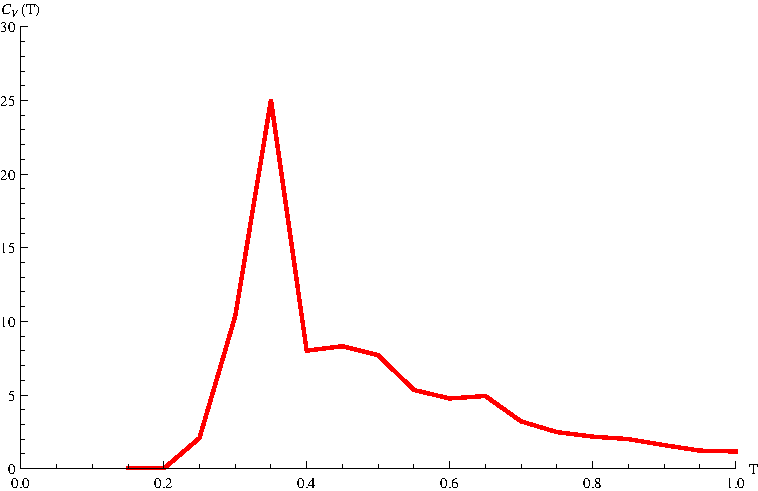
\includegraphics[width=.49\textwidth]{cv}
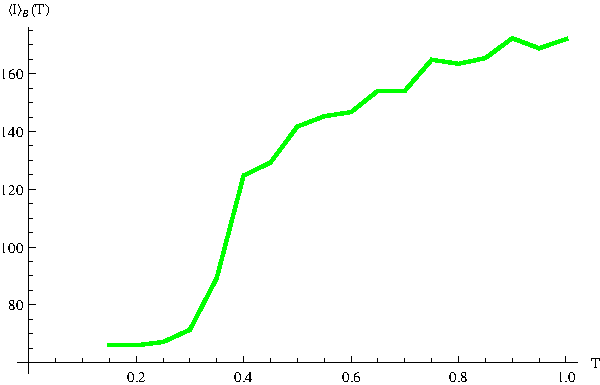
\includegraphics[width=.49\textwidth]{gyr}
\end{figure}


Przykładowy histogram wystąpień konfiguracji o~zadanej liczbie kontaktów przedstawiono na Rys.~4.3. %cos tu przestalo dzialac
\begin{figure}[h!]
\label{hist}
\caption[To należy zmienić]
{
Histogram kontaktów dla $T=0.35$, dla polimeru o~sekwencji\\PHPPHPPHHPPHHPPHPPHP:
}
\centering
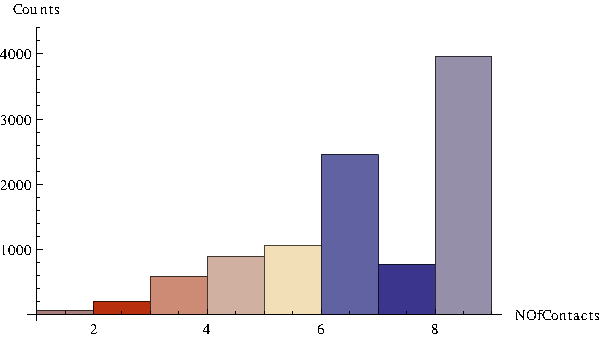
\includegraphics[width=.7\textwidth]{hist}
\end{figure}
\\

Wyniki należy przedstawić w~postaci
wykresów. Pisemne sprawozdania nie są obowiązkowe, sprawdzane będą wykresy (histogramy we wszystkich temperaturach, $C_V(T)$ i~$\langle I \rangle_B$(T)) i~działanie programu (na jednych z~ćwiczeń należy uruchomić program i~przeprowadzić symulacje).

\chapter{Trzeci program zaliczeniowy}
Celem trzeciego programu zaliczeniowego jest przeprowadzenie symulacji MD układu bardzo zbliżonego do znanego nam już modelu HP.
W pierwszej kolejności należy zaimplementować poniższy algorytm całkujący (\ref{BBK}).
Następnie, potrzebujemy upewnić się, że nasz program działa dla wymiarów wyższych, niż 1.
W końcu, musimy umożliwić, aby kilka potencjałów mogło opisywać nasz układ \emph{jednocześnie} (np. Lenarda-Jonesa + ``miękkie ścianki'')~--~w tym celu najlepiej jest skorzystać z dekoratora (wzorca projektowego omówionego na ćwiczeniach).
Warto dodać potencjał ``miękkie ścianki'', aby układ nie odpłynął nam w siną dal.
Jednak uwaga: stała $L$ powinna być na tyle duża, aby sfera zerowego potencjału pomieściła cały układ.

Do symulacji układu zbliżonego do modelu HP potrzebujemy jeszcze dwóch dodatkowych potencjałów: oddziaływania kolejnych aminokwasów i wiązania H--H (\ref{bonded} i \ref{morse}).
Dodatkowo, klasa \emph{Atom} potrzebuje nowego atrybutu~--~\emph{type}~--~który będzie znakiem P bądź H.
\section{Równanie Langevina - integrator BBK}
\label{BBK}
Oddziaływanie układu z termostatem o temperaturze $T$ modeluje się na wiele sposobów.
Jednym z nich jest integrator BBK:
\begin{displaymath}
\mathbf{r}(t+\Delta t) := \frac{2 \mathbf{r}(t) -\mathbf{r}(t-\Delta t)( 1 - \Delta t/2 ) + \frac{1}{m} ( \mathbf{F}(t) + \mathbf{F}_R ) (\Delta t)^2 }{1 + \Delta t / 2 },
\end{displaymath}
gdzie $\mathbf{F}_R$ jest siłą losową, generowaną z 3-wymiarowego rozkładu normalnego, ze średnią $\mathbf{0}$ i wariancją $2 k_B T m / \Delta t$ w każdym z trzech kierunków.
Przyjmujemy, że stała Boltzmanna ma wartość 1.

\section{Potencjał \emph{bonded}}
\label{bonded}
Jeżeli atomy $i$ oraz $j$ są kolejnymi elementami układu (``aminokwasami''), ich oddziaływnie wzbogacone będzie następującym potencjałem:
\begin{displaymath}
U(\mathbf{r}_{ij}) =  \kappa ( r_0 - ||\mathbf{r}_{ij}|| )^2 ,
\end{displaymath}
gdzie $\kappa$ jest stałą sprężystości (weźmy $\kappa=200$), $\mathbf{r}_{ij}$ to wektor łączący atom $i$ oraz $j$, zaś $r_0$ to odległość równowagowa między atomami (weźmy $r_0 = 1$).
Potencjał \emph{bonded} zapewniać będzie odpowiednią długość wiązania (u nas 1), tak aby nasz łańcuch przypominał model HP, w którym długość wiązań była ustalona ``na sztywno''.

\section{Potencjał Morse'a}
\label{morse}
Jeżeli atomy $i$ oraz $j$ są typu H i dzielą je co najmniej dwa inne atomy (tzn. \mbox{$|i-j|>2$}), występuje między nimi oddziaływanie H--H, które modelować będziemy potencjałem Morse'a:
\begin{displaymath}
U(\mathbf{r}_{ij}) = D \hspace{0.1cm} (1 - e^{ -\alpha ( || \mathbf{r}_{ij} || - r_0) })^2 - D,
\end{displaymath}
w którym stała $D$ wpływa na głębokość minimum, zaś parametr $\alpha$ na kształt (``stromość'') funkcji.
Weźmiemy $D=1$ oraz $\alpha=20$.
\begin{figure}[h!]
\label{potencjal}
\caption[To należy zmienić]
{
Kształt potencjałów: Lenarda-Jonesa ($\mathcal{E},R=1$), Morse'a ($D=1$, $\alpha = 20$) oraz \emph{bonded} ($\kappa = 200$) w przypadku 1-wymiarowym.
}
\centering
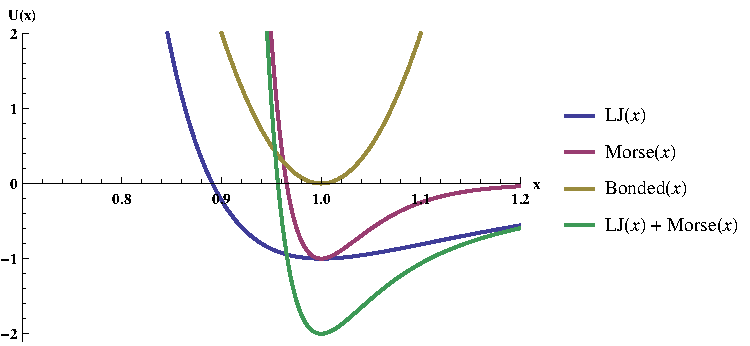
\includegraphics[scale=0.9]{potentials}
\end{figure}

\section{Symulacja}
Zaliczenie trzeciego programu zaliczeniowego polegać będzie na przeprowadzeniu symulacji przy zadanej długości i liczbie kroków.
Na stałe można wszyć do programu: układ i algorytm całkujący (BBK).
Prosiłbym, aby układem wyjściowym był pierwszy łańcuch HP z drugiego programu zaliczeniowego, z konfiguracją o najniższej energii.
Przedział temperatur, który nas interesuje to $T\in[0,1]$.

W odróżnieniu do pierwszego programu zaliczeniowego, tym razem sprawdzana będzie przede wszystkim trajektoria układu (plik {\tt .xyz}).


\addcontentsline{toc}{chapter}{Bibliografia}
\begin{thebibliography}{99}

\bibitem{unfolded}
A.~L.~Fink.
\newblock {\em Natively unfolded proteins,}
\newblock Curr Opin Struct Biol {\bf 15}, 35–41.
\\

Najczęściej cytowana w~branży dynamiki molekularnej pozycja:
\bibitem{understanding}
D.~Frenkel, B.~Smit.
\newblock {\em Understanding Molecular Simulation – From Algorithms to Applications,} volume~1~of {\em Computational Science Series.}
\newblock Academic Press, A~Division of Harcourt, Inc., 2nd edition, 2002.
\\

Świetne wprowadzenie do fizycznych podstaw dynamiki molekularnej (lepsze od Frenkela\&Smita, zdaniem autora tego skryptu):
\bibitem{zuckerman}
D. M. Zuckerman.
\newblock {\em Statistical Physics of Biomolecules: An Introduction,}
\newblock CRS PRESS, 2010.
\\

Praca, którą będziemy omawiać w~ramach II programu zaliczeniowego:
\bibitem{dill}
K. A. Dill.
\newblock {\em Principles of protein folding—a perspective from simple exact models,}
\newblock Protein Science, vol. 4, no. {\bf 4}, pp. 561–602, 1995.
\\

Strona kursu dynamiki molekularnej (dobry opis algorytmów termostatowych):
\bibitem{dobraStronka}
Cameron Abrams.
\newblock \texttt{www.pages.drexel.edu/\textasciitilde cfa22/msim/msim.html}
\newblock {\em Department of Chamical Engineering, Drexel University, Philadelphia.}

	
\end{thebibliography}


\end{document}
